\section{Addestramento}
I modelli di Machine Learning scelti per affrontare il problema sono quattro:
albero decisionale, Multi Layer Perceptron, Support Vector Machine e
Gaussian Naive Bayes classifier.
I primi tre modelli sono stati scelti in quanto, in base all'esperienza
maturata nell'intera
industria, essi si rivelano spesso performanti su feature estratte da immagini,
come avviene in questo caso.
Il quarto modello, ovvero Gaussian Naive Bayes, è stato invece scelto per provare
un approccio probabilistico al problema, e studiarne le performance. Inoltre,
anche Gaussian Naive Bayes si rivela essere molto spesso un buon classificatore
per feature estratte da immagini.

\subsection{Albero decisionale}
Un albero decisionale è un modello di Machine Learning che cerca di 
costruire un albero di classificazione. Ogni nodo interno corrisponde alla scelta
di una feature e al partizionamento dello spazio delle istanze associato in un 
numero di sottoinsiemi pari al numero di valori da essa assunti se la feature
è discreta, due se la feature è continua.
In questo ultimo caso, il primo sottoinsieme contiene le istanze il cui valore 
assunto dalla feature scelta è minore della sua media, mentre il secondo contiene
tutte le altre.
Le foglie rappresentano, invece, i nodi in cui viene effettivamente
effettuata la classificazione, in quanto a ognuna di esse è associata una classe.
Si può notare che, quando si trattano feature continue, la stessa feature può
essere usata più volte in uno stesso cammino radice-foglia.

La selezione di una feature per un certo nodo interno avviene in modo tale che 
essa sia quella che massimizza il miglioramento di una certa metrica 
se calcolata sul partizionamento definito dai suoi nodi figli. 
Esistono due metriche per la valutazione delle feature: indice di Gini ed entropia
di Shannon.

Per stabilire quale criterio permette di definire l'albero decisionale
migliore per il dataset che si sta considerando, si effettua una grid search
su entrambi i criteri, e si considera il modello con il maggiore macro-f1 score.
Per contenere la complessità dell'albero (e quindi l'overfitting), inoltre,
vengono valutati anche i parametri associati alla profondità massima
e al numero di foglie massimo.
I criteri di separazione che vengono valutati sono: \begin{itemize*}
    \item indice di Gini
    \item entropia di Shannon
\end{itemize*}.
I valori di profondità massima valutati sono: \begin{itemize*}
    \item 6
    \item 8
    \item 10
\end{itemize*}.
Il numero massimo di foglie può invece assumere i valori: \begin{itemize*}
    \item 20
    \item 25
    \item 35
\end{itemize*}.

A seguito della grid search, il modello migliore si rivela essere quello la cui
combinazione di parametri è criterio = Gini, profondità massima = 8 e numero massimo
di foglie = 35.

Le performance del modello si rivelano essere ottime: si riscontrano 
un macro-f1 score del $91,3\%$, una macro-precisione del $91\%$ e 
un macro-recall del $91\%$.

\begin{Figure}
    \centering
    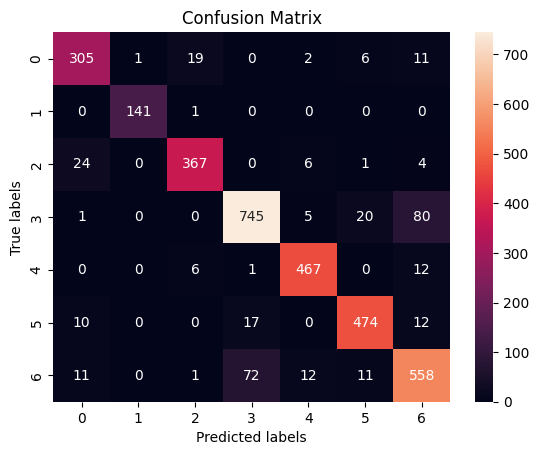
\includegraphics[width=\linewidth]{img/tree_confusion_matrix.png}
    \captionof{figure}{Matrice di confusione dell'albero decisionale.}
\end{Figure}

\subsection{Multi Layer Perceptron}
Un Multi Layer Perceptron è una rete neurale feed-forward fully connected in cui 
ogni neurone si comporta come un percettrone. Una rete neurale è composta
da diversi strati di neuroni, che possono essere suddivisi in: strato di input;
strati nascosti; strato di output.
Un percettrone di uno strato nascosto attiva la sua connessione in output
sse il suo input pesato supera una certa soglia, detta soglia di attivazione.
L'apprendimento della rete avviene tramite la modifica dei pesi definiti
sulle connessioni tra neuroni: durante l'addestramento, la rete neurale esegue,
a intervalli regolari definiti dalla batch size, la backpropagation, ovvero
aggiorna i suoi pesi in modo tale da ridurre, idealmente, l'errore di previsione.
Per propagare l'errore, e quindi aggiornare i pesi, la rete usa la discesa del
gradiente, basata sulle derivate prime della funzione errore. Inoltre,
la discesa del gradiente richiede che le funzioni di attivazione dei neuroni
siano derivabili.
Le funzioni di attivazione derivabili più utilizzate sono lineare, tanh, relu
e softmax (solitamente usata per il layer di output). Alcune di esse, come tanh,
sono più computazionalmente onerose rispetto alle altre.
Ogni rete neurale, inoltre, esamina l'input per un certo numero di epoche:
una singola analisi dell'intero dataset di addestramento corrisponde a un'epoca.

La complessità di una rete neurale, e di conseguenza il suo overfitting, cresce
all'aumentare del numero di layer e del numero di neuroni contenuti in un
singolo layer: la rete deve quindi
essere definita in modo da ottenere alte performance con un numero limitato
di layer e neuroni per layer.
Un altro fattore di overfitting può essere l'esecuzione di molte epoche.

Per trovare la combinazione di parametri migliore per la rete, viene eseguita 
una grid search. 
I valori considerati per numero di layer layer e numero di nodi per layer sono:
\begin{itemize*}
    \item $(5, 5)$
    \item $(10)$
\end{itemize*}.
Le funzioni di attivazione considerate sono invece: \begin{itemize*}
    \item tanh
    \item relu
\end{itemize*}.

\begin{Figure}
    \centering
    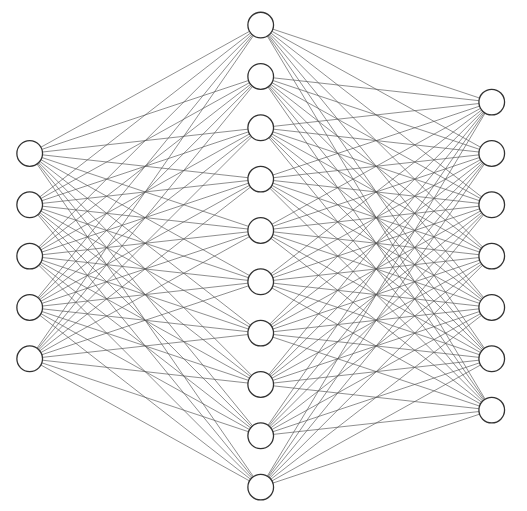
\includegraphics[width=0.8\linewidth]{img/mlp.png}
    \captionof{figure}{Multi Layer Perceptron con i parametri migliori.}
\end{Figure}

A seguito della grid search, la combinazione di parametri migliore si rivela essere 
layer = $(10)$ e funzione di attivazione = relu.

Le performance sono ottime: si rileva un macro-f1 score del $93,8\%$, 
una macro-precisione del $94\%$ e un macro-recall del $94\%$.

\begin{Figure}
    \centering
    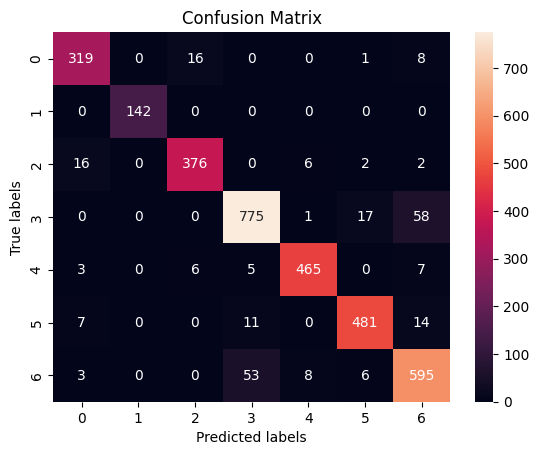
\includegraphics[width=\linewidth]{img/mlp_low_confusion_matrix.png}
    \captionof{figure}{Matrice di confusione del MLP.}
\end{Figure}

La complessità della rete rimane comunque elevata: analizzando la loss curve
definita nel corso dell'addestramento, infatti, si può evidenziare il fatto
che la loss non decresce significativamente per un elevato numero di epoche,
aumentando il rischio di overfitting sui dati di training e richiedendo un maggiore
tempo di addestramento. L'addestramento termina, quindi, al limite stabilito
dalla libreria Sklearn, ovvero 200 epoche.

\begin{Figure}
    \centering
    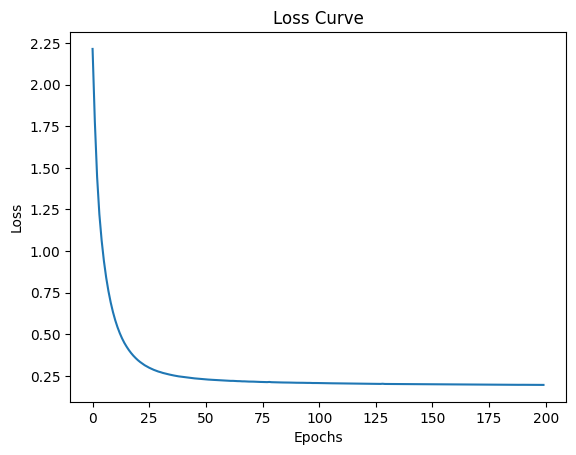
\includegraphics[width=0.9\linewidth]{img/mlp_low_loss.png}
    \captionof{figure}{Loss curve del MLP.}
\end{Figure}

Una tecnica che può essere utilizzata per ridurre il numero di epoche
è quella di aumentare la tolleranza della rete.
La tolleranza è, infatti, un parametro che stabilisce un decremento minimo
della loss durante l'esecuzione del training: se per 5 epoche la loss
diminuisce di un valore minore della tolleranza, allora il training si può
arrestare.
La tolleranza individuata che permette di mantenere performance simili alla
precedente rete è tol = 0.001. Rieffettuando il training, si può osservare che 
il numero di epoche si riduce a circa 80, dimezzando di fatto il numero
di epoche richieste.

\begin{Figure}
    \centering
    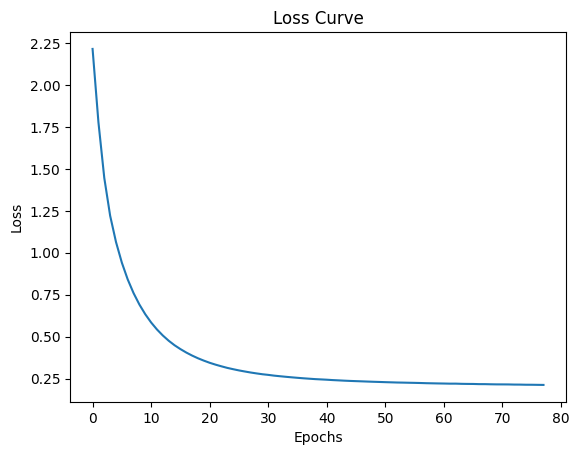
\includegraphics[width=0.9\linewidth]{img/mlp_high_loss.png}
    \captionof{figure}{Loss curve del MLP con tol = 0.001.}
\end{Figure}

\begin{Figure}
    \centering
    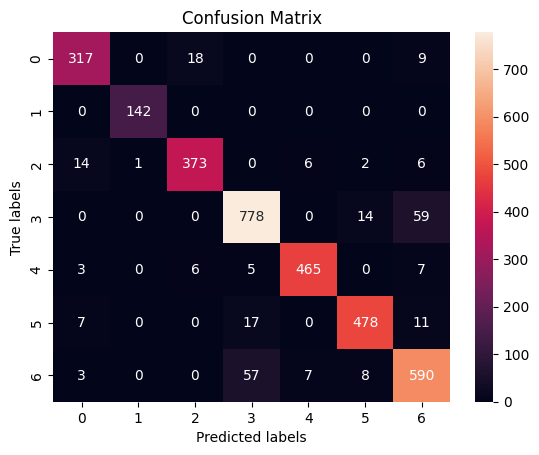
\includegraphics[width=\linewidth]{img/mlp_high_confusion_matrix.png}
    \captionof{figure}{Matrice di confusione del MLP con tol = 0.001.}
\end{Figure}

Le performance della rete con una maggiore tolleranza sono anch'esse ottime:
si rileva un macro-f1 score del $93,5\%$, 
una macro-precisione del $94\%$ e un macro-recall del $93\%$.

\subsection{Support Vector Machine}
Una Support Vector Machine è un modello di Machine Learning fortemente legato
al concetto di separabilità delle istanze: durante il suo addestramento, infatti,
essa cerca di separarle utilizzando degli iperpiani, in modo che istanze
appartenenti alla stessa classe ricadano nella stessa regione di spazio. 
Il numero di iperpiani di separazione necessari per classificare $n$ classi
è pari a $n-1$: in questo caso, quindi, saranno necessari 6 iperpiani, in quanto
le varietà di fagioli considerate sono 7.

L'apprendimento di una SVM "pura" converge, però, sse le istanze
sono linearmente separabili.
Esistono quindi due tecniche che permettono di trattare anche dataset non linearmente
separabili: soft-margin e kernel trick.

La prima tecnica, il soft-margin, consiste nel tollerare una certa quantità di
errore, e permettere quindi una misclassificazione di un numero ridotto di
istanze. La quantità di errore tollerata viene determinata da un parametro $C$,
detto trade-off, che deve essere stabilito prima dell'apprendimento.
Al crescere di $C$, l'errore tollerato si riduce e la complessità del modello
aumenta.

Il kernel trick permette, invece, di separare le istanze utilizzando funzioni non
lineari. In realtà, il kernel trick non separa le istanze con vere e proprie
funzioni non lineari, ma le separa linearmente in uno spazio di dimensione
maggiore di quello di partenza; questo 
iperpiano, però, si traduce in una funzione non lineare nello spazio di partenza.
Anche in questo caso, la funzione kernel da utilizzare deve essere stabilita prima dell'apprendimento.
Le funzioni kernel più comuni sono: \begin{itemize*}
    \item lineare
    \item polinomiale
    \item radial basis function (rbf).
\end{itemize*}

Prima di procedere con l'addestramento, è necessario anche effettuare un'osservazione
sulle scale delle feature: una SVM è, infatti, sensibile a feature con diverse scale,
e risulta più performante su dataset a cui è stato applicato lo scaling.
Questo passaggio è, però, già stato effettuato nella fase di Analisi esplorativa.

Viene quindi eseguita una grid search per individuare la combinazione di parametri
migliore, ovvero quella che massimizza il macro-f1 score.
I valori di trade-off considerati sono: \begin{itemize*}
    \item 1
    \item 2
    \item 5
\end{itemize*}.
I kernel considerati sono invece: \begin{itemize*}
    \item lineare
    \item polinomiale
    \item radial basis function (rbf)
\end{itemize*}.

\begin{Figure}
    \centering
    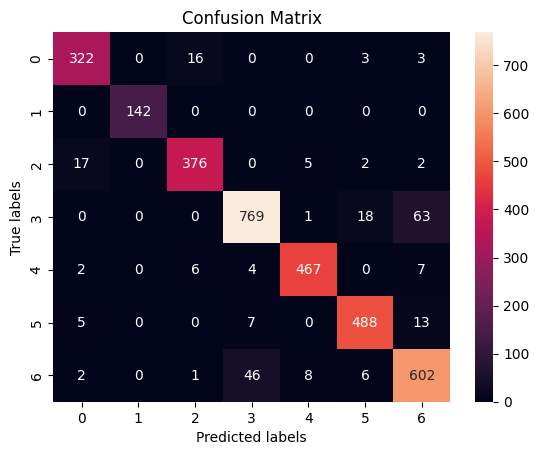
\includegraphics[width=\linewidth]{img/svm_confusion_matrix.png}
    \captionof{figure}{Matrice di confusione della SVM.}
\end{Figure}

A seguito della grid search, la combinazione migliore si rivela essere $C=2$ e
kernel = rbf. Di conseguenza, la complessità del modello è abbstanza contenuta,
grazie al basso valore di $C$.
Il numero di vettori di supporto individuati da questa SVM è pari a 2153.

Le perfomance della SVM addestrata con questi parametri sono ottime:
si rivela un macro-f1 score del $94,1\%$, 
una macro-precisione del $94\%$ e un macro-recall del $94\%$.

\subsection{Gaussian Naive Bayes}
Gaussian Naive Bayes classifier è un modello di Machine Learning basato sul
teorema di Bayes: a ogni nuova istanza di addestramento analizzata, infatti,
il modello aggiorna le probabilità delle classi usando proprio il teorema di Bayes.
La classificazione avviene, invece, scegliendo la classe di probabilità maggiore
data l'istanza che si vuole classificare.
Gaussian Naive Bayes è la variante del Naive Bayes classifier che può essere applicata
a dataset con feature continue (Naive Bayes può infatti trattare solo feature 
discrete) e con valori negativi.

Questo classificatore si può utilizzare solo facendo alcune
assunzioni: la distribuzione di probabilità di ogni feature deve essere
normale e ogni feature deve essere condizionalmente indipendente dalle altre.
Per quanto riguarda la prima assunzione, le componenti principali del dataset
hanno tutte distribuzioni normali, escluse la prima e la seconda che, invece,
presentano una distribuzione multimodale. 
Esse si possono comunque assumere normali, in modo da poter ugualmente applicare il 
classificatore gaussiano.

\begin{Figure}
    \centering
    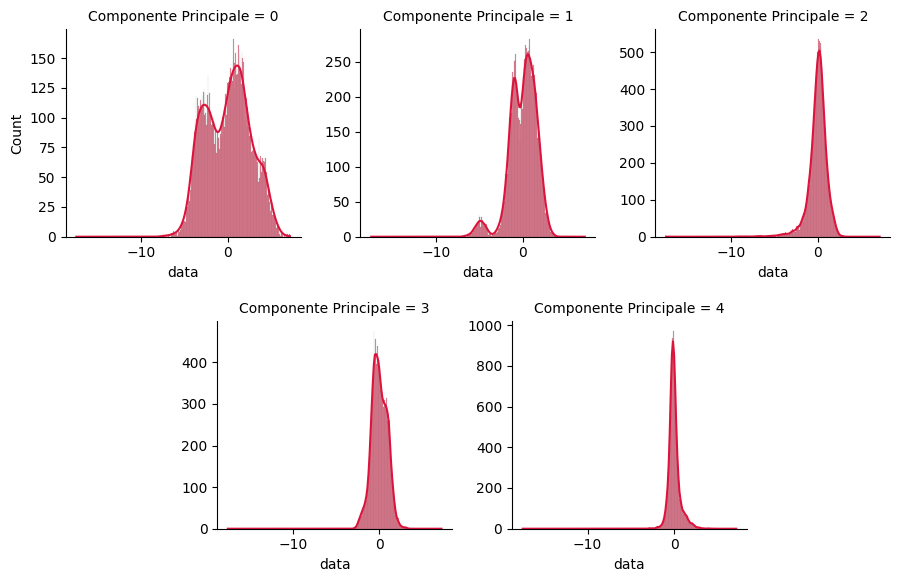
\includegraphics[width=\linewidth]{img/components_distribution.png}
    \captionof{figure}{Distribuzioni di probabilità per le componenti principali
    considerate.}
\end{Figure}

Inoltre, tutte le feature con varianza 0 non devono essere considerate, in quanto
non portano alcuna informazione e non permettono al classificatore di 
raggiungere performance ottimali. Si può osservare, però, che le uniche feature
rimaste sono le 5 componenti principali scelte da PCA, ognuna con varianza
strettamente maggiore di 0.

\begin{Figure}
    \centering
    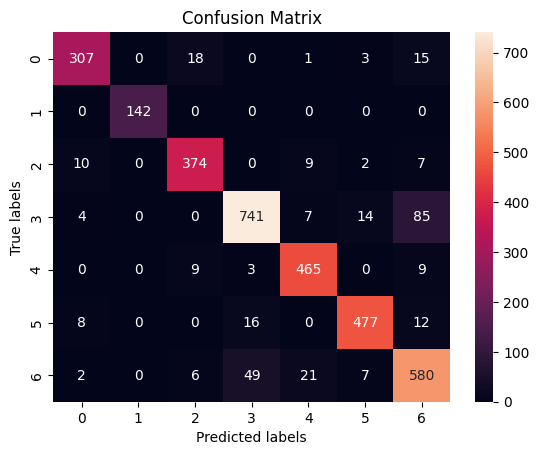
\includegraphics[width=\linewidth]{img/gnb_confusion_matrix.png}
    \captionof{figure}{Matrice di confusione di Gaussian Naive Bayes.}
\end{Figure}

Nonostante tutte queste assunzioni, il classificatore gaussiano si rivela essere
molto performante e velocissimo da addestrare:
si rileva un macro-f1 score del $92,1\%$, 
una macro-precisione del $92\%$ e un macro-recall del $92\%$.
